\section{Application Implementation and Documentation}
In questa sezione sono esposte la struttura del progetto, le dipendenze software del progetto, le strutture dati implementate per il DB, le API implementate con diversi diagrammi.

\subsection{Project Structure}
Per il progetto abbiamo volute dividere lo sviluppo del front-end e del back-end in due cartelle separate in modo da dividerci i compiti in maniera più facile e appropriata. Nel Back-end abbiamo le seguenti cartelle:

\begin{figure}[!h]
\centering
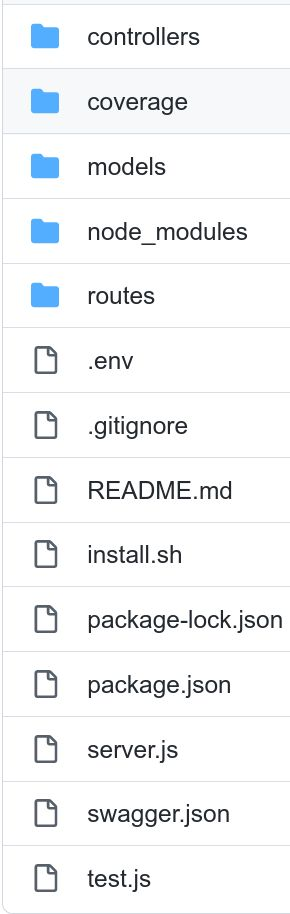
\includegraphics[scale=0.3]{images/struttura_back-end.jpg}
\caption{Struttura Back-end }
\label{fig:struttura_back}
\end{figure}
\noindent
Nella cartella \textbf{models}, abbiamo definito tutte le strutture dati che il database deve essere in grado di manipolare. \\
Nella cartella \textbf{routes} abbiamo definito tutti gli end-point delle API che abbiamo sviluppato. \\
Nella cartella \textbf{controllers} abbiamo inserito la definizione di questi end-point e quindi il vero e proprio codice, che viene eseguito all'invocazione delle API. \\
La cartella \textbf{coverage} è una cartella generata automaticamente in fase di testing dell'applicazione. \\
\\
\newpage
Nel Front-end abbiamo le seguenti cartelle:

\begin{figure}[!h]
\centering
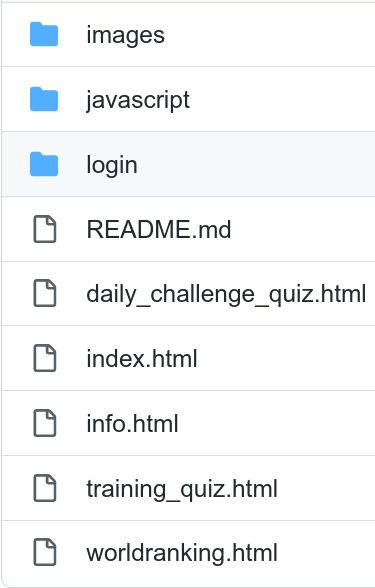
\includegraphics[scale=0.3]{images/struttura_front-end.jpg}
\caption{Struttura Front-end }
\label{fig:struttura_front-end}
\end{figure}
\noindent
Nella cartella \textbf{images} abbiamo tutte le immagini utilizzate nel Front-end. \\
Nella cartella \textbf{javascript} sono contenuti tutti gli script javascript delle diverse pagine. \\
Nella cartella \textbf{login} sono presenti le pagine HTML per il login. \\
Nella root della cartella Front-end sono contenute invece tutte le altre pagine HTML.

\subsection{Project Dependencies}
I seguenti moduli Node sono stati utilizzati e aggiunti al file 'package.json': 
\begin{itemize}
    \item \textbf{cors}: necessario per connettere Back-end con Front-end ed effettuare le chiamate alle API con successo.
    \item \textbf{dotenv}: necessario per utilizzare le variabili d'ambiente.
    \item \textbf{express}: necessario per setuppare un server.
    \item \textbf{jest-fetch-mock}: necessario per effettuare il testing finale dell'applicazione.
    \item \textbf{mongoose-express-api}: necessario per connettersi al database MongoDB.
    \item \textbf{nodemailer}: necessario per inviare e-mail.
    \item \textbf{swagger-ui-express}: necessario per produrre la documentazione con swagger.
\end{itemize}

\subsection{Project Data or DB}
Per la gestione dei dati utili all’applicazione sono state definite quattro strutture dati: quiz, sfida giornaliera, simbolo, e utente.
\begin{figure}[!h]
\centering
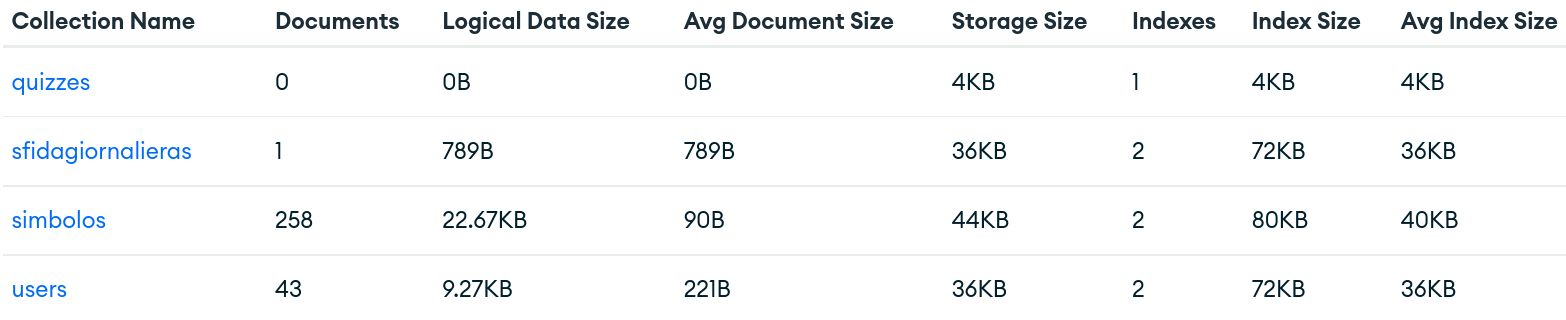
\includegraphics[scale=0.35]{images/project_data_db.jpg}
\caption{Collezione dati usati nell'applicazione}
\label{fig:struttura_front-end}
\end{figure}
\noindent

\newpage
\noindent
Definizione degli schemi delle diverse strutture dati:
\begin{figure}[!h]
\centering
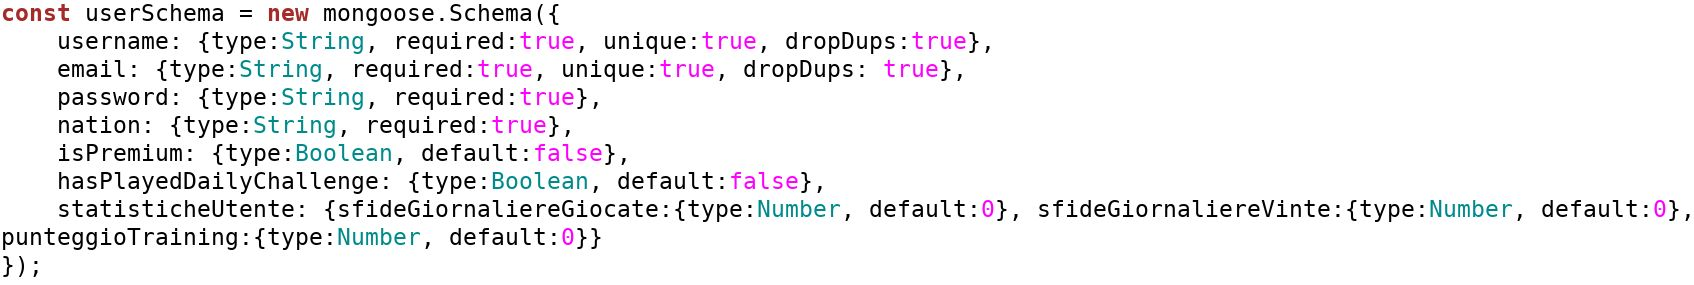
\includegraphics[scale=0.35]{images/user_schema_db.jpg}
\caption{Schema definito per l'utente}
\label{fig:user_schema_db}
\end{figure}
\noindent

\begin{figure}[!h]
\centering
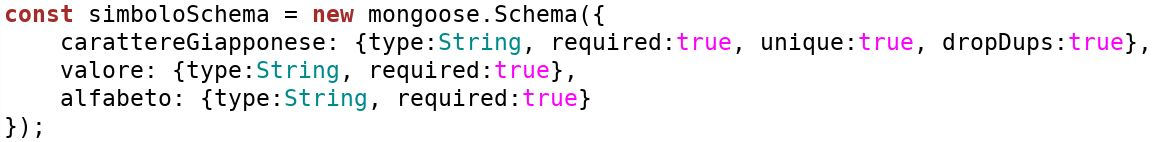
\includegraphics[scale=0.35]{images/simbolo_schema_db.jpg}
\caption{Schema definito per il simbolo}
\label{fig:simbolo_schema_db}
\end{figure}
\noindent

\begin{figure}[!h]
\centering
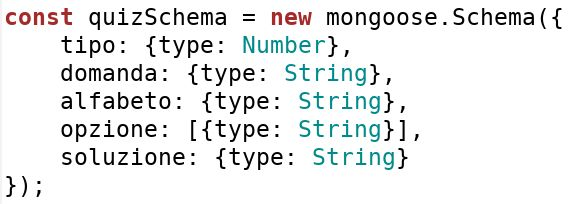
\includegraphics[scale=0.35]{images/quiz_schema_db.jpg}
\caption{Schema definito per il quiz}
\label{fig:quiz_schema_db}
\end{figure}
\noindent

\begin{figure}[!h]
\centering
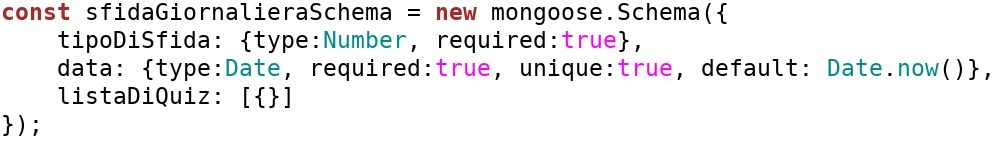
\includegraphics[scale=0.35]{images/sfida_giornaliera_schema_db.jpg}
\caption{Schema definito per la sfida giornaliera}
\label{fig:sfida_giornaliera_schema_db}
\end{figure}
\noindent


\subsection{Project APIs}
\subsubsection{Resources Extraction from the Class Diagram}
Nel diagramma delle classi possiamo notare diverse "risorse" (tipi di dati con relativi metodi nativi del nostro programma). A diverse di queste risorse sono associate delle API che svolgono determinati ruoli all'interno del progetto. In questo diagramma vengono espresse prima le risorse (come Utente, Quiz o Sfida Giornaliera) e sotto di loro collegate tramite frecce le rispettive API. \\
Ogni API è caratterizzata dal tipo ( POST / PATCH / GET), da degli eventuali parametri di cui ha bisogno per funzionare e infine da un riferimento Front-end o Back-end, a seconda del ruolo che svolge l'API, se principalmente di front-end o di back-end. \\
Nel nostro progetto la risorsa con più API è chiaramente Utente, infatti abbiamo bisogno di API quali login, signup, nuova e-mail per tutte quelle funzionalità che riguardano il profilo dell'utente. Abbiamo in aggiunta anche delle API strettamente legate al progetto stesso come la visualizzazione della classifica o delle proprie statistiche, o il passaggio a premium per poter usare il training Kanji. 
\begin{figure}[!h]
\centering
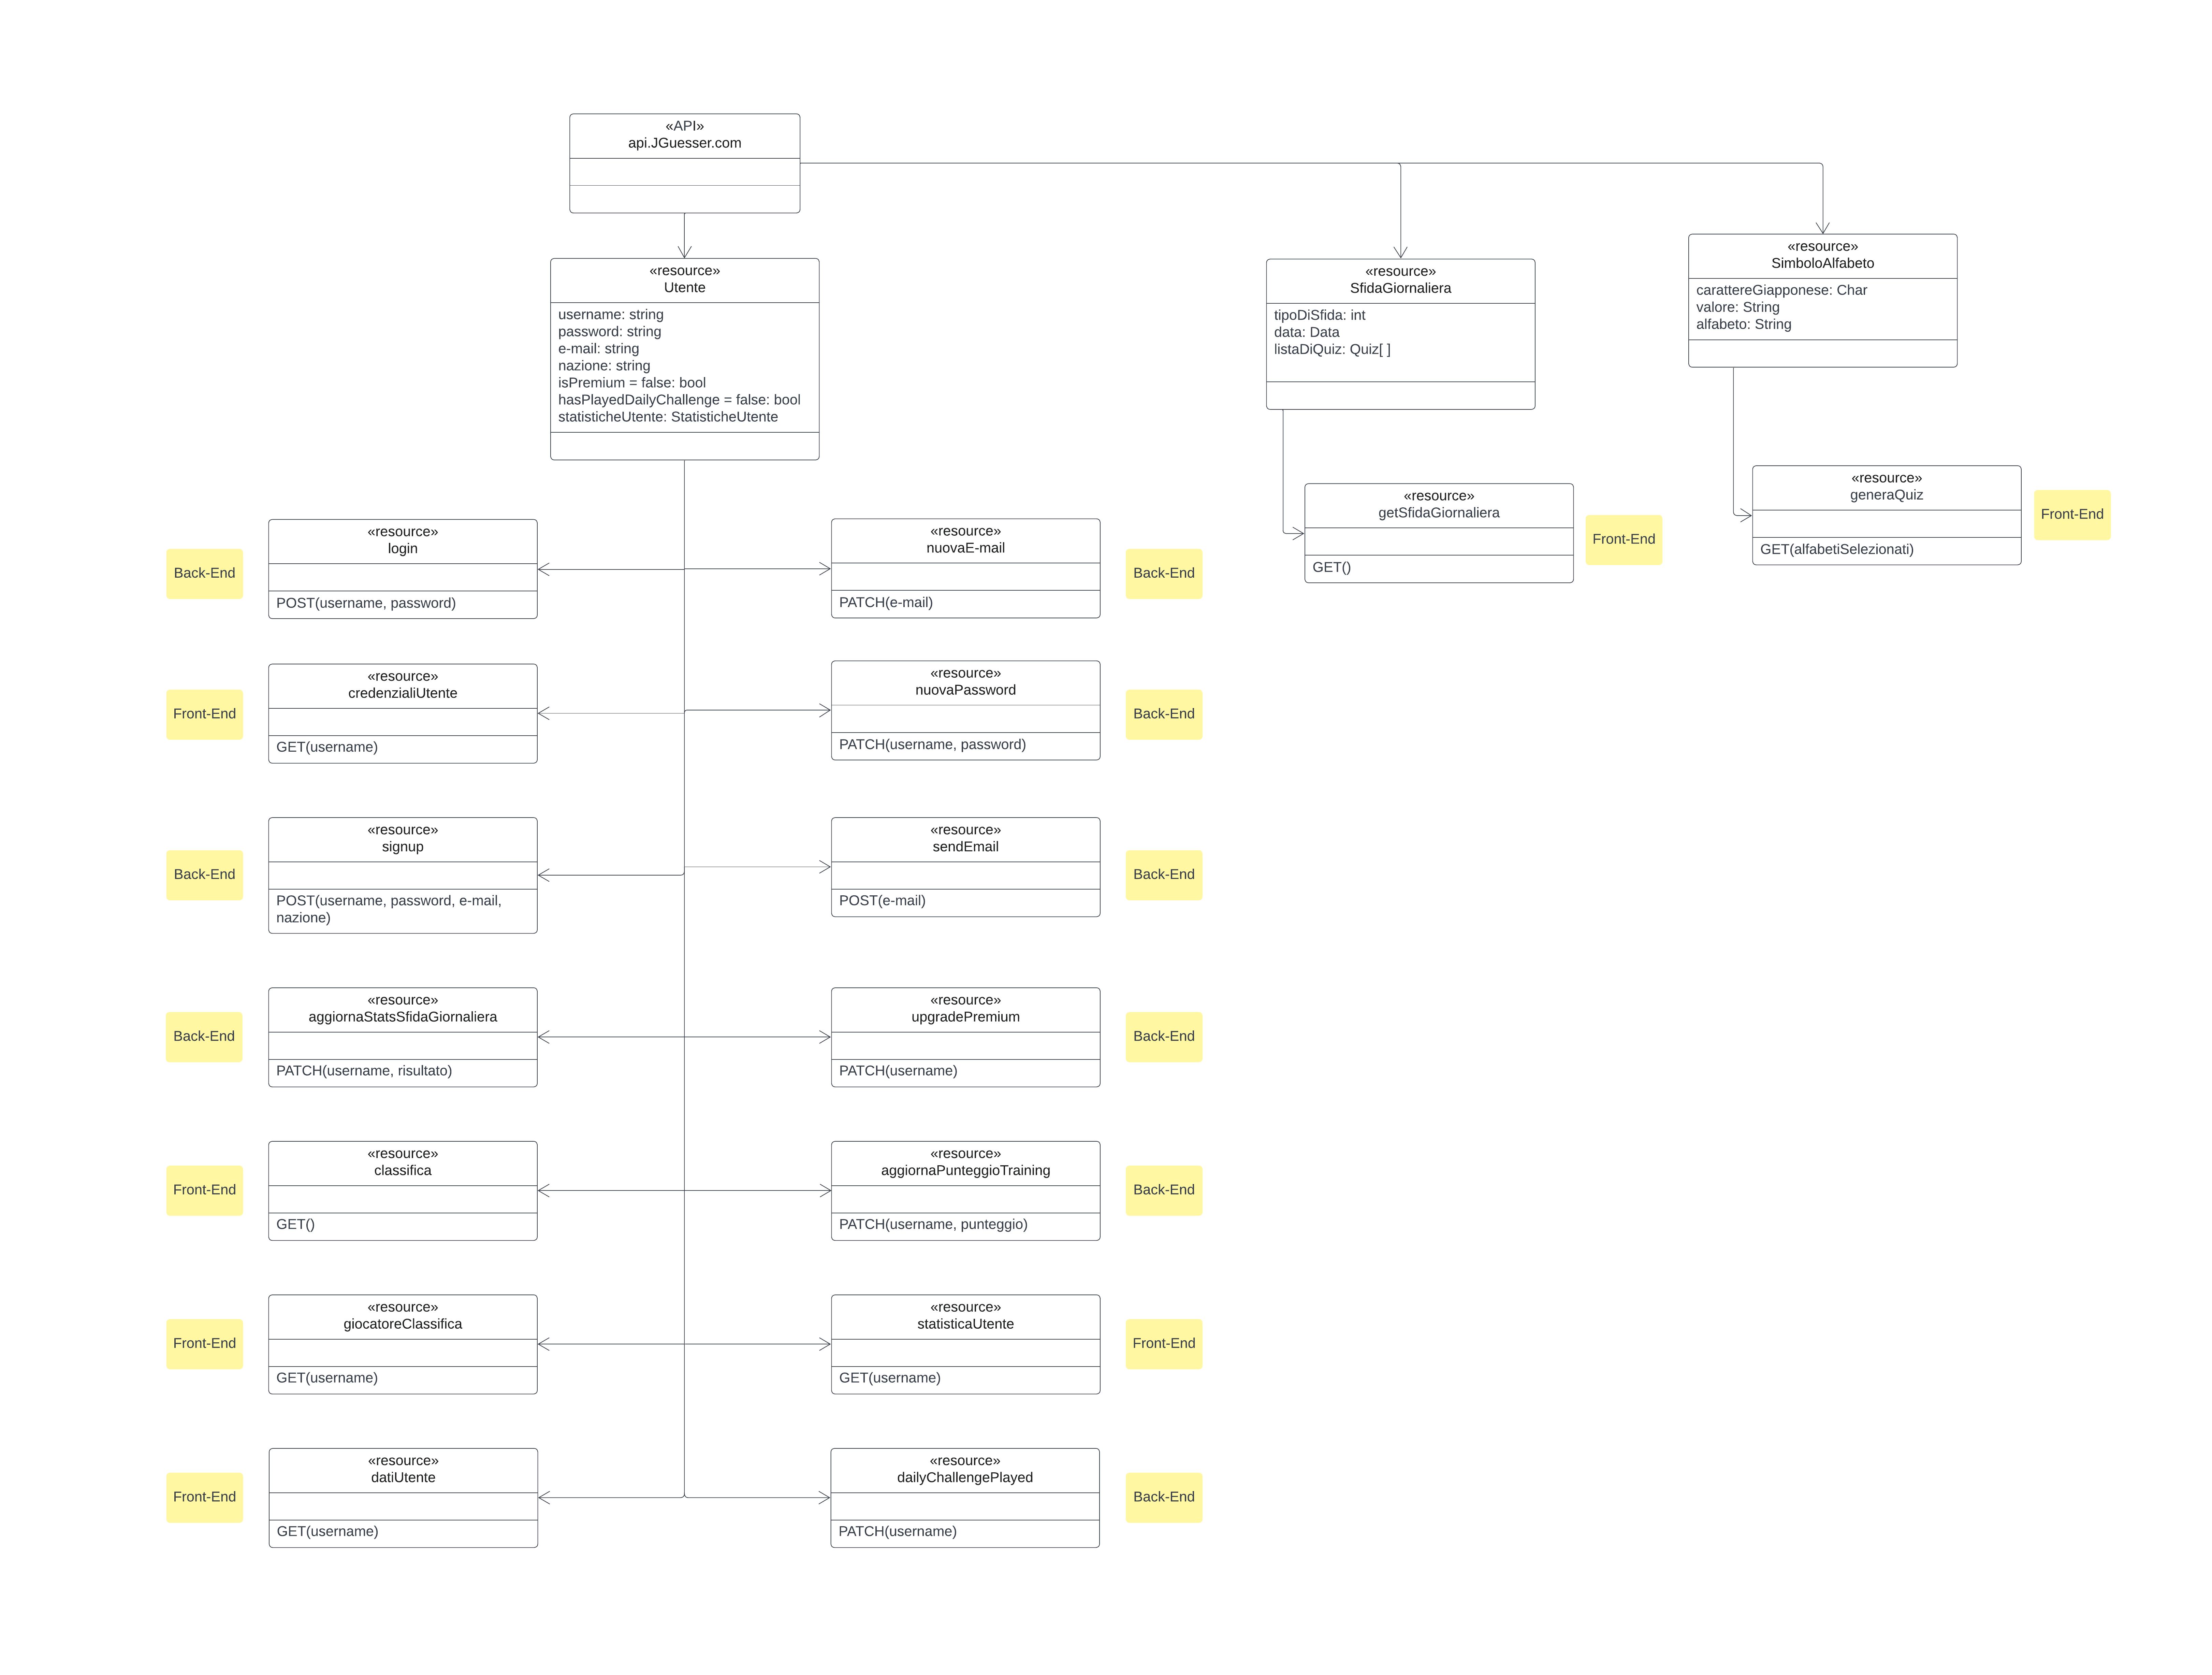
\includegraphics[scale=0.05]{images/From Class Diagram to API implementation.png}
\caption{Diagramma "Resources Extraction form Class Diagram"}
\label{fig:From Class Diagram to API implementation.png}
\end{figure}

\subsubsection{Resources Models}
Nel diagramma delle risorse sono spigate nel dettaglio tutte le API del progetto, dal percorso interno a "routes" al nome dell'API e ai singoli casi di input e output. Abbiamo rispettato le convenzioni "HTML" per i messaggi di stato individuando nel nostro progetto diversi stati possibili per diverse API. Quelli più comuni sono il 404 NOT FOUND, 200 OK, 304 NOT MODIFIED e 500 INTERNAL SERVER ERROR. La maggioranza delle API non ha bisogno di un body di input ma solamente di parametri passati nell'URI. Un caso paticolare nel nostro progetto è il logout visto che non è stato necessario implementare un'API apposita grazie al tipo di implementazione dell'autenticazione e della registrazione (tramite localStorage). 
\begin{figure}[!h]
\centering
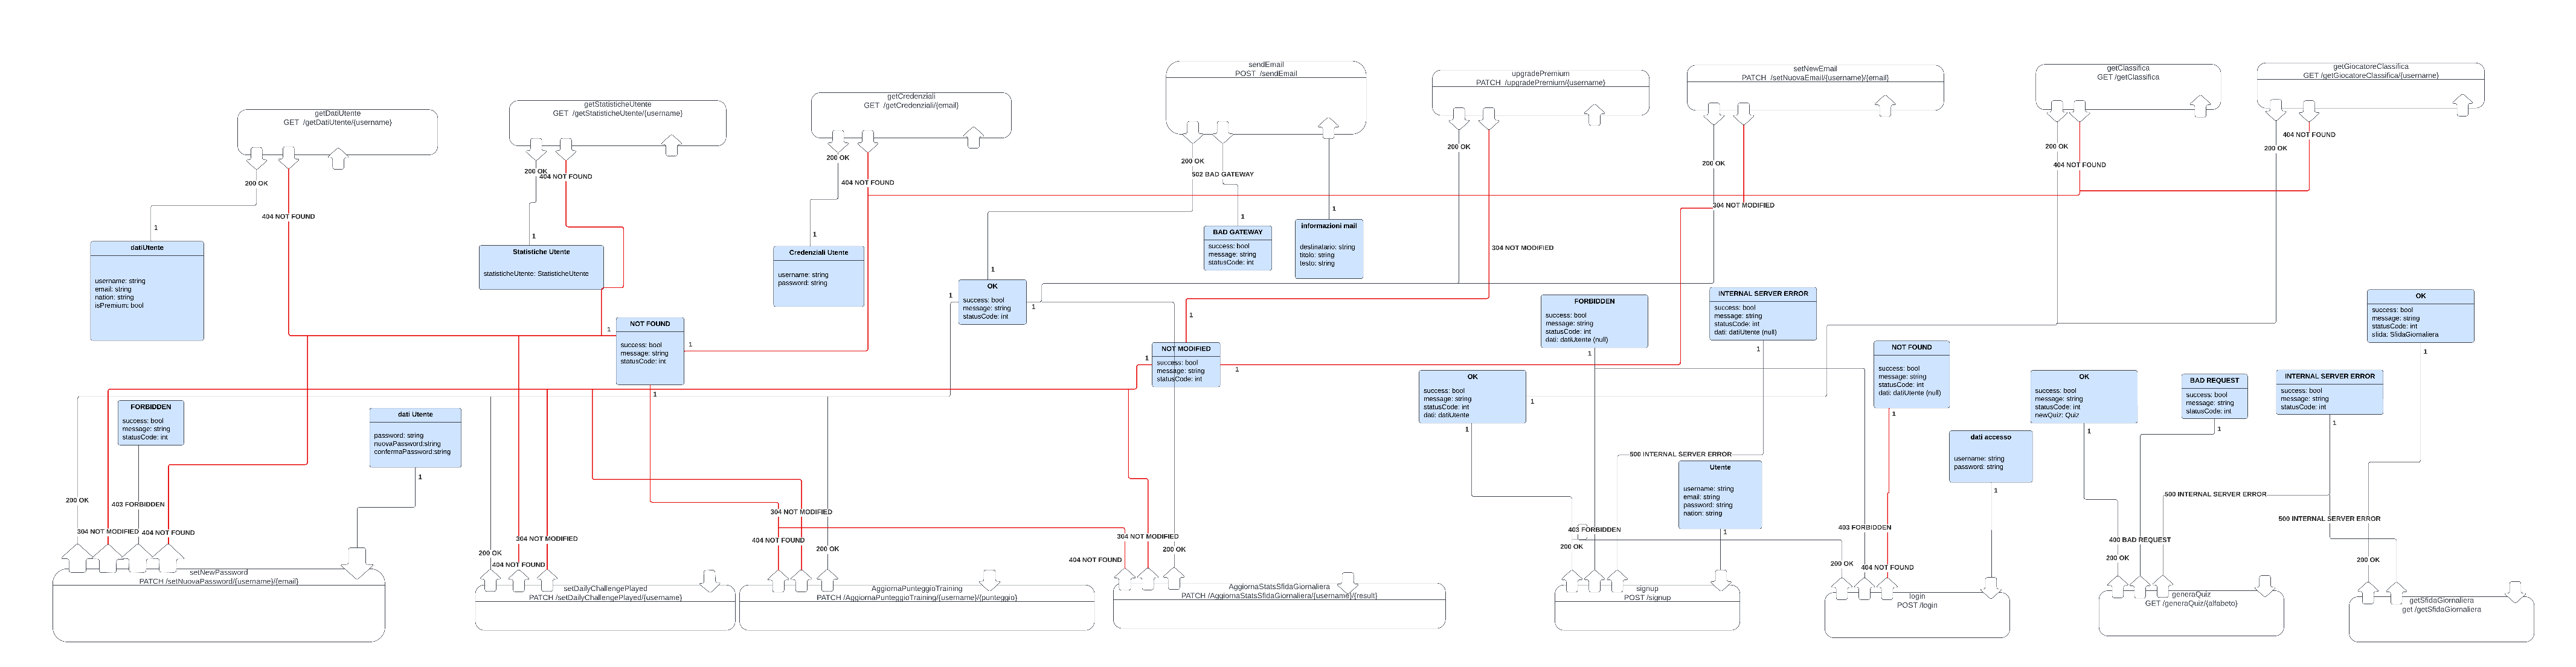
\includegraphics[scale=0.1]{images/Resources Diagram.png}
\caption{Diagramma delle Risorse}
\label{fig:Resources Diagram.png}
\end{figure}

\newpage
\subsection{Sviluppo API}
In questa sezione sono descritte le varie API che abbiamo sviluppato.

\subsubsection{Registrazione}
\begin{figure}[!h]
\centering
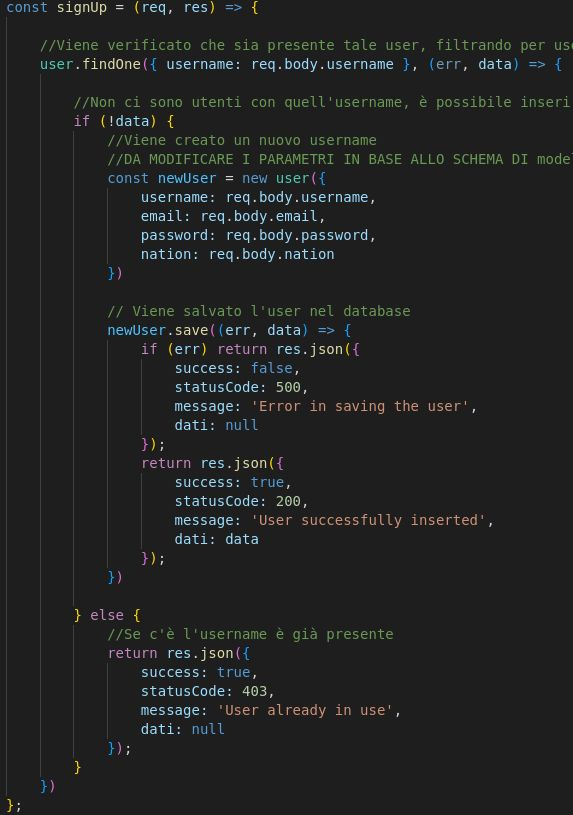
\includegraphics[scale=0.4]{images/api_signup.jpg}
\caption{Implementazione API signUp}
\label{fig:api_signup}
\end{figure}
\noindent
Questa API di tipo POST permette all'utente di registrarsi. I parametri richiesti per registrare un utente sono:
\begin{itemize}
    \item username;
    \item e-mail;
    \item password;
    \item nation.
\end{itemize}
Questa API restituisce un codice:
\begin{itemize}
    \item 200: la registrazione è avvenuta con successo e vengono restituiti anche i dati di registrazione;
    \item 403: l'utente non può essere registrato perchè esiste gia un account con quel username;
    \item 500: errore generico, che significa che ci è stato un errore lato server nel salvare i dati nel database.
\end{itemize}

\newpage
\subsubsection{Autenticazione}
\begin{figure}[!h]
\centering
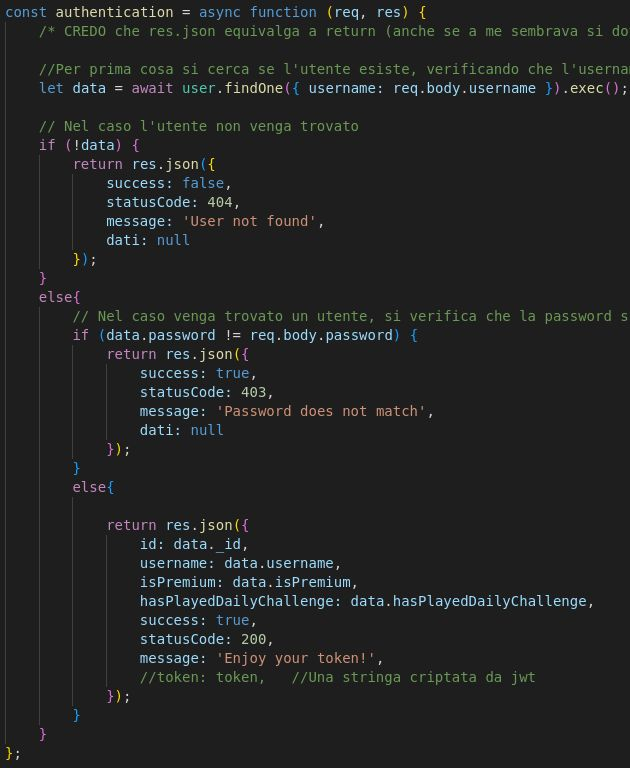
\includegraphics[scale=0.4]{images/api_authentication.jpg}
\caption{Implementazione API login}
\label{fig:api_authentication}
\end{figure}
\noindent
Questa API di tipo POST permette all'utente di autenticarsi. I parametri richiesti per autenticare un utente sono:
\begin{itemize}
    \item username;
    \item password.
\end{itemize}
Questa API restituisce un codice:
\begin{itemize}
    \item 200: l'autenticazione è avvenuta con successo e vengono restituiti una serie di dati necessari per l'utene;
    \item 403: la password che l'utente ha inserito non corrisponde alla password memorizzata all'interno del database;
    \item 404: non c'è nessun utente con quello specifico username.
\end{itemize}

\subsubsection{Mostra classifica}
\begin{figure}[!h]
\centering
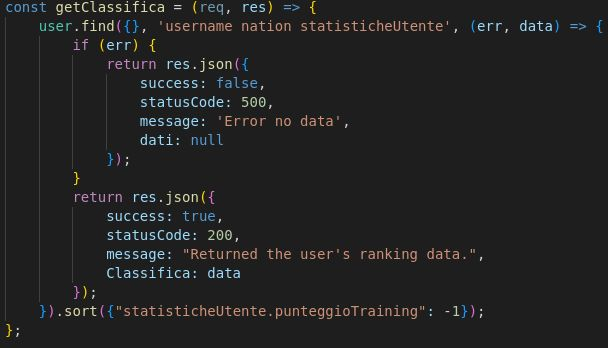
\includegraphics[scale=0.4]{images/api_classifica.jpg}
\caption{Implementazione API classifica}
\label{fig:api_classifica}
\end{figure}
\noindent
Questa API di tipo GET restituisce tutti i dati della classifica in ordine decrescente di punteggio training. 
Questa API restituisce un codice:
\begin{itemize}
    \item 200: i dati sono stati restituiti correttamente;
    \item 500: c'è stato un errore lato server e non si è riuscito a restituire i dati.
\end{itemize}

\subsubsection{Ricerca dati classifica di uno specifico giocatore}
\begin{figure}[!h]
\centering
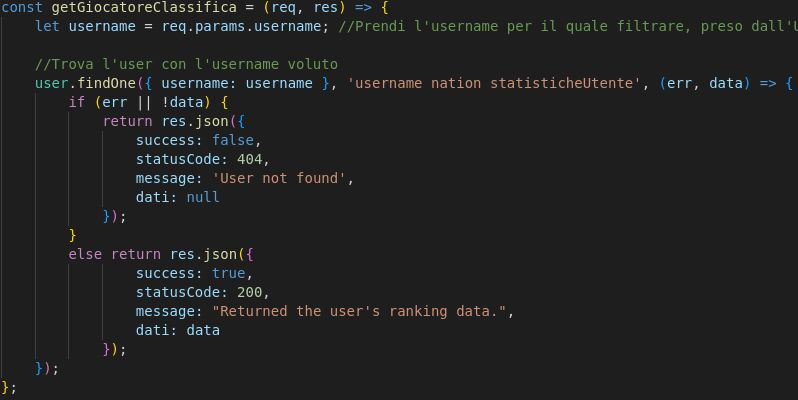
\includegraphics[scale=0.4]{images/api_giocatore_classifica.jpg}
\caption{Implementazione API giocatore classifica}
\label{fig:api_giocatore_classifica}
\end{figure}
\noindent
Questa API di tipo GET restituisce tutti i dati della classifica di uno specifico giocatore. È richiesto di inserire nell'url della richiesta l'username del giocatore che si intende cercare.
Questa API restituisce un codice:
\begin{itemize}
    \item 200: l'utente è stato trovato e se ne restituiscono i dati da visualizzare;
    \item 404: non c'è nessun utente con quello specifico username.
\end{itemize}

\subsubsection{Ottieni i dati di uno specifico utente}
\begin{figure}[!h]
\centering
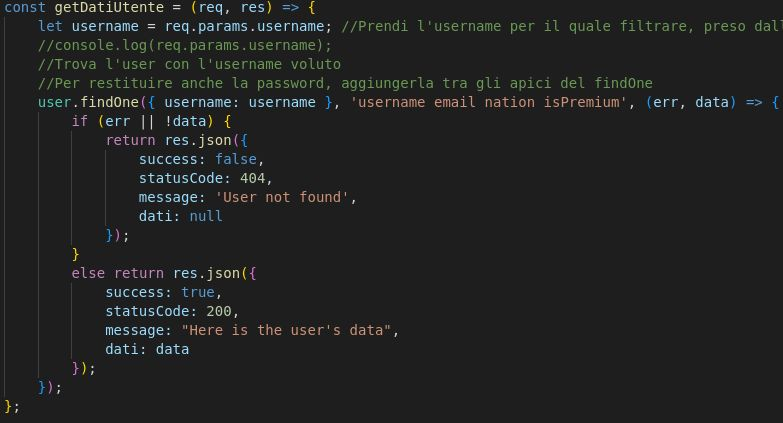
\includegraphics[scale=0.4]{images/api_dati_utente.jpg}
\caption{Implementazione API dati utente}
\label{fig:api_dati_utente}
\end{figure}
\noindent
Questa API di tipo GET restituisce i dati di uno specifico utente. Per dati di uno specifico utente si intende: 
\begin{itemize}
    \item username;
    \item e-mail;
    \item nation;
    \item isPremium.
\end{itemize}
Sono in sostanza quelli che sono visualizzati nella prima parte della propria pagina profilo. Questa API restituisce un codice:
\begin{itemize}
    \item 200: l'utente è stato trovato e se ne restituiscono i dati da visualizzare;
    \item 404: non c'è nessun utente con quello specifico username.
\end{itemize}

\subsubsection{Ottieni le credenziali di un utente data la sua e-mail}
\begin{figure}[!h]
\centering
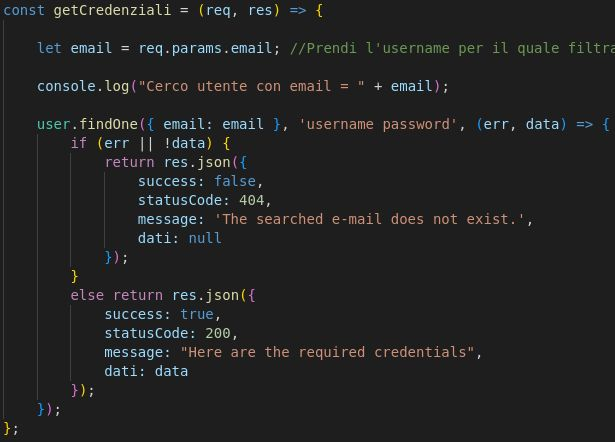
\includegraphics[scale=0.4]{images/api_credenziali.jpg}
\caption{Implementazione API credenziali}
\label{fig:api_credenziali}
\end{figure}
\noindent
Questa API di tipo GET restituisce le credenziali di uno specifico utente data l'e-mail associata.
Questa API restituisce un codice:
\begin{itemize}
    \item 200: l'utente è stato trovato e se ne restituiscono username e password;
    \item 404: non c'è nessun utente con quella specifica e-mail.
\end{itemize}

\subsubsection{Ottieni le statistiche di uno specifico utente}
\begin{figure}[!h]
\centering
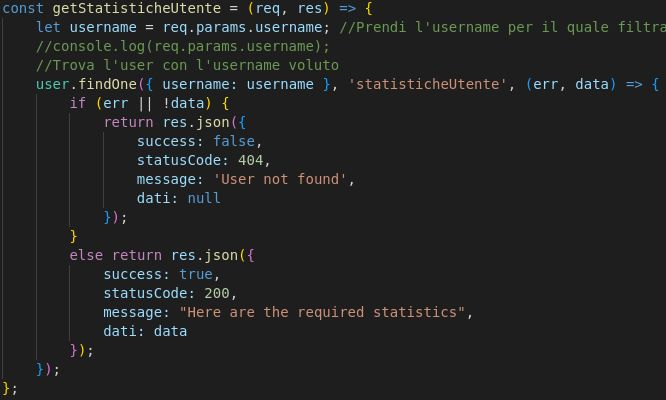
\includegraphics[scale=0.4]{images/api_statistiche_utente.jpg}
\caption{Implementazione API statistiche utente}
\label{fig:api_statistiche_utente}
\end{figure}
\noindent
Questa API di tipo GET restituisce le statistiche di uno specifico utente.
Questa API restituisce un codice:
\begin{itemize}
    \item 200: l'utente è stato trovato e se ne restituisco le statistiche;
    \item 404: non c'è nessun utente con quello specifico username.
\end{itemize}

\newpage
\subsubsection{Invia un e-mail tramite JGuesser}
\begin{figure}[!h]
\centering
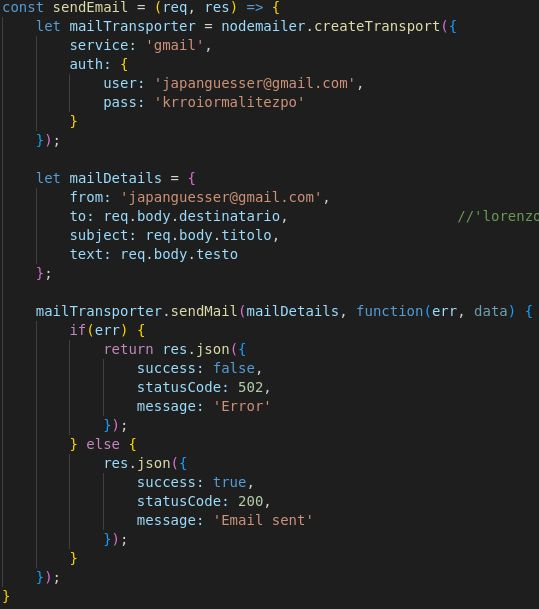
\includegraphics[scale=0.4]{images/api_send_email.jpg}
\caption{Implementazione API send e-mail}
\label{fig:api_send_email}
\end{figure}
\noindent
Questa API di tipo POST prende come parametri in input nel body:
\begin{itemize}
    \item destinatario: e-mail di destinazione.
    \item titolo: oggetto dell'e-mail;
    \item testo: contenuto dell'e-mail.
\end{itemize}
e invia con l'indirizzo e-mail 'japanguesser@gmail.com' un e-mail con le specifiche appena descritte.
Questa API restituisce un codice:
\begin{itemize}
    \item 200: l'e-mail è stata inviata con successo;
    \item 502: non è stato possibile inviare l'e-mail.
\end{itemize}

\subsubsection{Impostazione di una nuova e-mail}
\begin{figure}[!h]
\centering
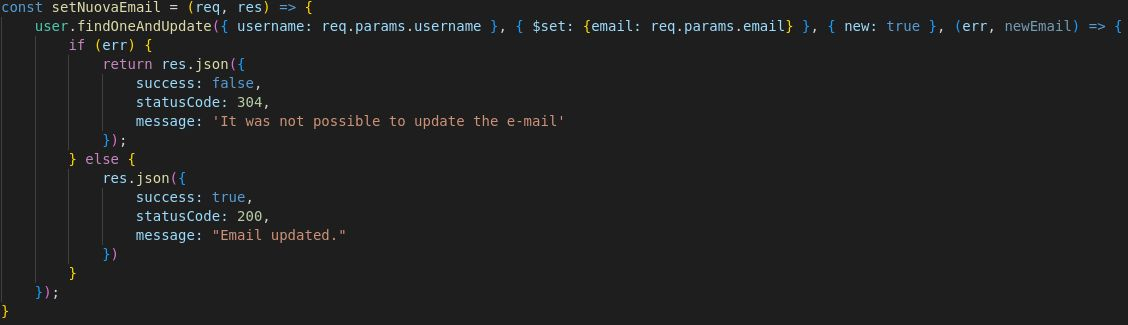
\includegraphics[scale=0.4]{images/api_nuova_email.jpg}
\caption{Implementazione API nuova e-mail}
\label{fig:api_nuova_email}
\end{figure}
\noindent
Questa API di tipo PATCH prende come parametri nell'URL l'username con la nuova e-mail da settare e modifica l'e-mail dell'utente.
Questa API restituisce un codice:
\begin{itemize}
    \item 200: l'utente è stato trovato e l'e-mail è stata modificata con successo;
    \item 304: c'è stato un errore e non è stato possibile modificare la risorsa.
\end{itemize}

\newpage
\subsubsection{Impostazione di una nuova password}
\begin{figure}[!h]
\centering
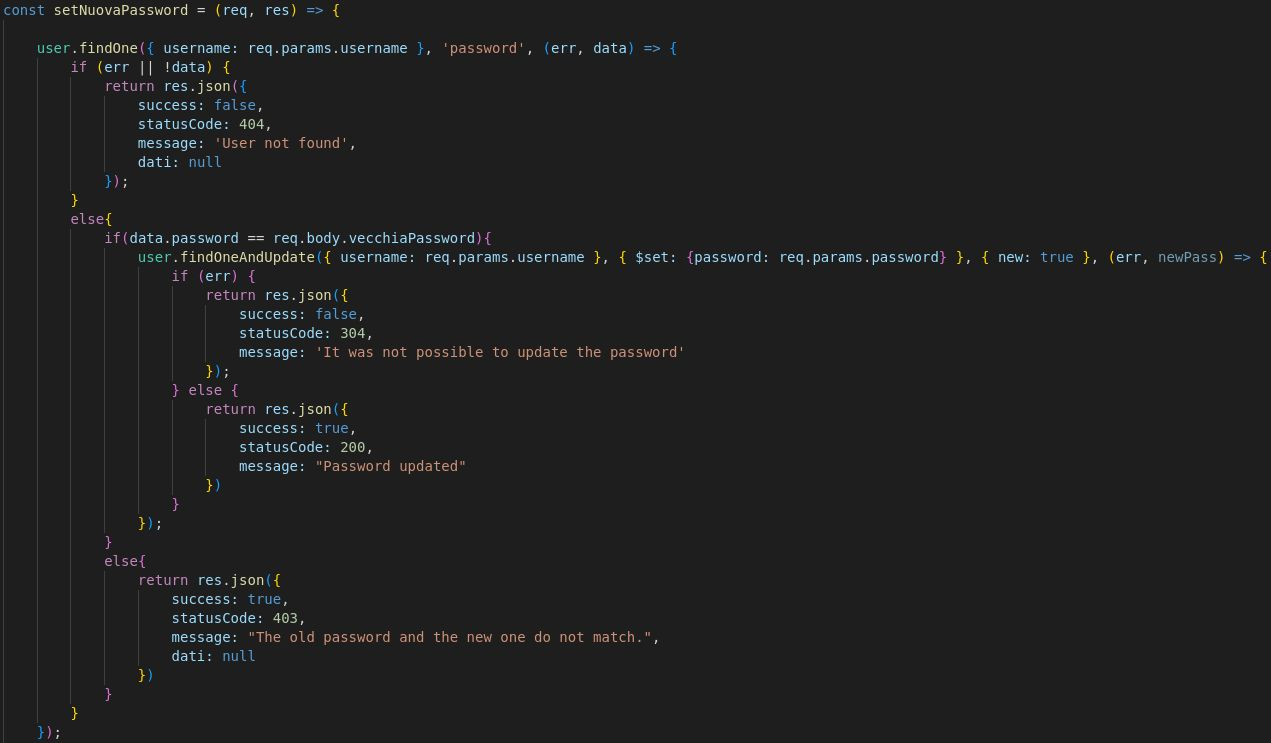
\includegraphics[scale=0.4]{images/api_nuova_password.jpg}
\caption{Implementazione API nuova password}
\label{fig:api_nuova_password}
\end{figure}
\noindent
Questa API di tipo PATCH prende come parametri nell'URL l'username con la nuova password da settare e nel body la vecchia password. Quello che fa è controllare che la vecchia password corrisponda a quella memorizzata nel database e poi va a settare quella nuova.
Questa API restituisce un codice:
\begin{itemize}
    \item 200: l'utente esiste, la password vecchia corrisponde e il server è riuscito a settare la nuova password;
    \item 304: c'è stato un errore e non è stato possibile modificare la risorsa;
    \item 404: l'utente non esiste e quindi non è possibile fare alcuna modifica;
    \item 403: la vecchia password inserita e quella presente sul database non corrispondono.
\end{itemize}

\subsubsection{Upgrade dell'utente a premium}
\begin{figure}[!h]
\centering
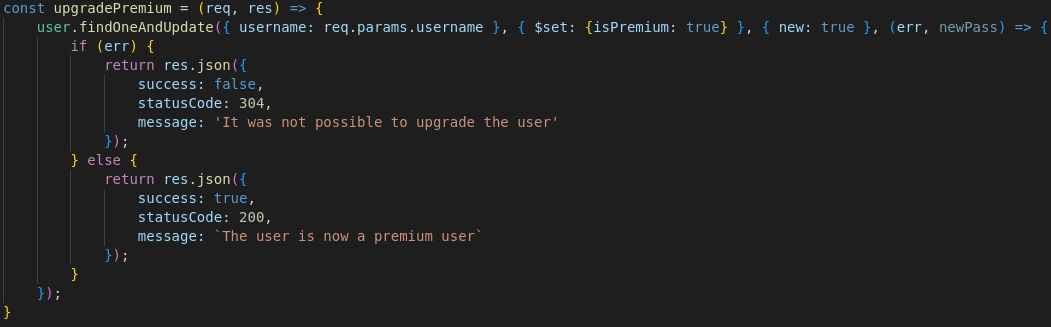
\includegraphics[scale=0.4]{images/api_upgrade_premium.jpg}
\caption{Implementazione API upgrade premium}
\label{fig:api_upgrade_premium}
\end{figure}
\noindent
Questa API di tipo PATCH prende come parametri nell'URL l'username dell'utente a cui verrà effettuato l'upgrade a premium.
Questa API restituisce un codice:
\begin{itemize}
    \item 200: i privilegi dell'utente sono stati aggiornati con successo;
    \item 304: c'è stato un errore e non è stato possibile modificare la risorsa.
\end{itemize}

\subsubsection{Impostazione daily challenge giocata}
\begin{figure}[!h]
\centering
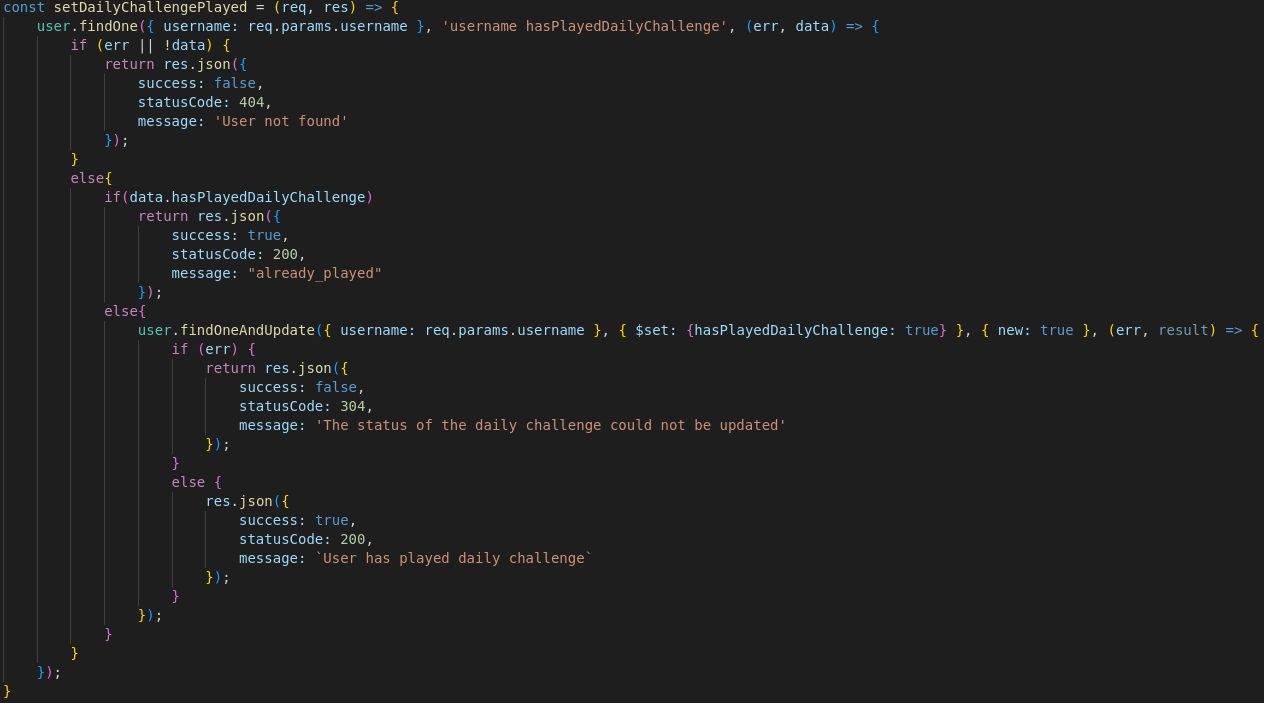
\includegraphics[scale=0.4]{images/api_set_daily_challenge.jpg}
\caption{Implementazione API impostazione challenge}
\label{fig:api_set_daily_challenge}
\end{figure}
\noindent
Questa API di tipo PATCH prende come parametri nell'URL l'username dell'utente a cui verrà settata la daily challenge come giocata. Nel caso in cui questo l'abbia gia giocata viene restituito il messaggio 'already\_played'.
Questa API restituisce un codice:
\begin{itemize}
    \item 200: significa che hasPlayedDailyChallenge è settato a true o è stato trovato, gia settato a 'true';
    \item 304: c'è stato un errore e non è stato possibile modificare la risorsa.
    \item 404: l'utente per il quale si vuole eseguire questa operazione non esiste.
\end{itemize}

\newpage
\subsubsection{Aggiornamento punteggio training}
\begin{figure}[!h]
\centering
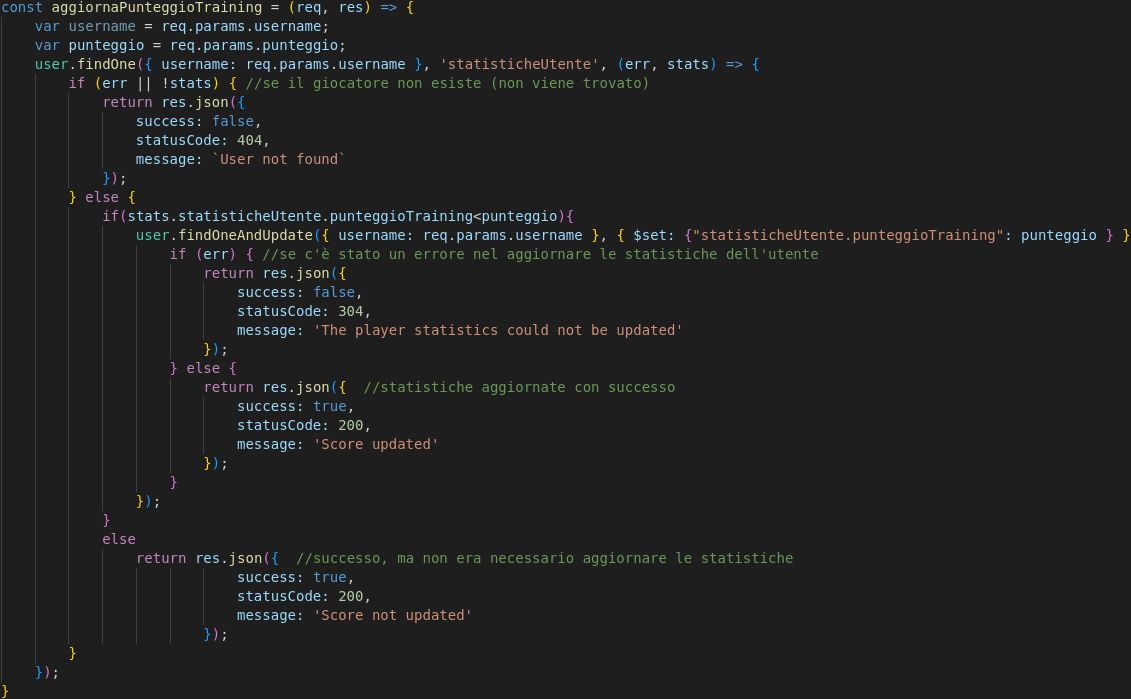
\includegraphics[scale=0.4]{images/api_aggiorna_punteggio_training.jpg}
\caption{Implementazione API aggiorna punteggio training}
\label{fig:api_aggiorna_punteggio_training}
\end{figure}
\noindent
Questa API di tipo PATCH prende come parametri nell'URL l'username dell'utente e il nuovo punteggio raggiunto nel training. Quello che questa API fa è aggiornare il massimo punteggio raggiunto nel training del giocatore.
Questa API restituisce un codice:
\begin{itemize}
    \item 200: significa che questa operazione di controllo e in caso di aggiornamento è avvenuta con successo;
    \item 304: c'è stato un errore e non è stato possibile modificare la risorsa;
    \item 404: l'utente per il quale si vuole potenzialmente aggiornare il proprio punteggio non esiste.
\end{itemize}

\newpage
\subsubsection{Aggiornamento punteggio sfida giornaliera}
\begin{figure}[!h]
\centering
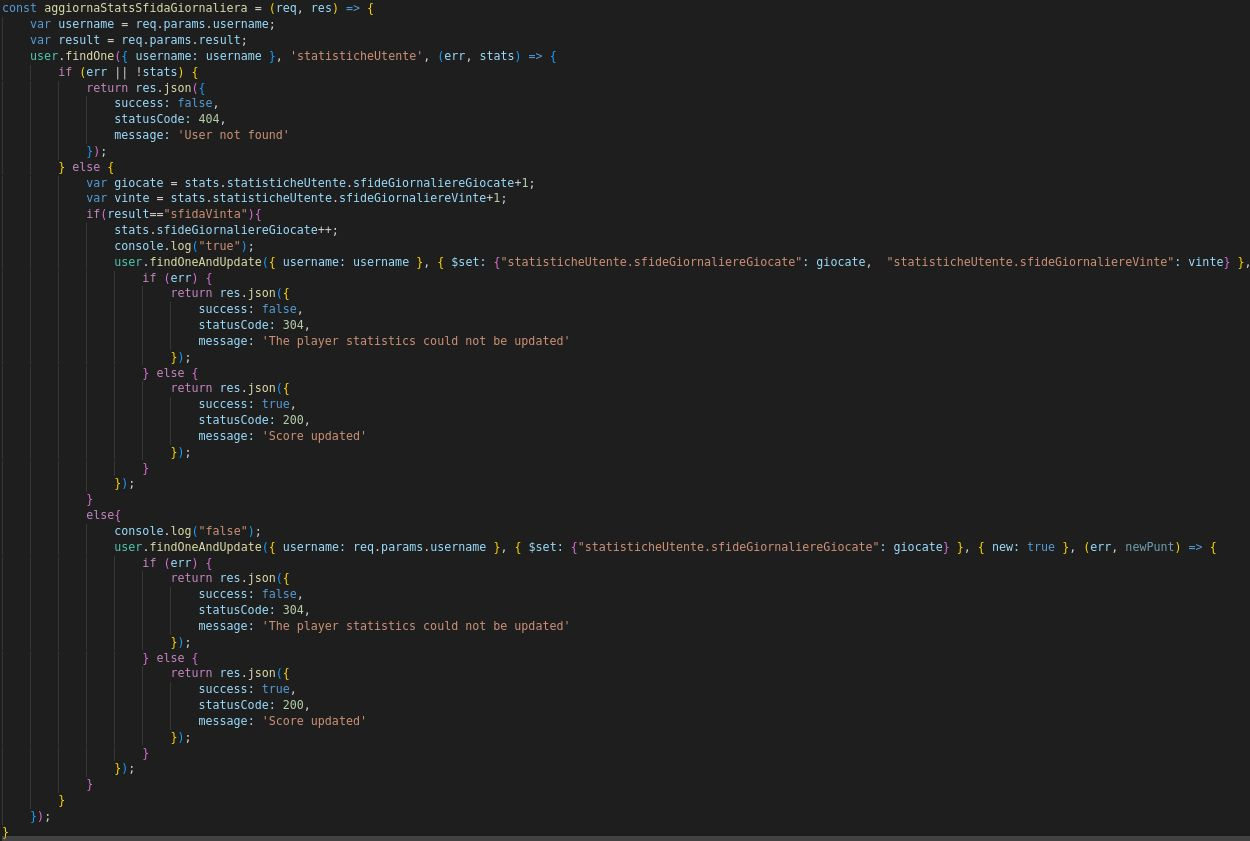
\includegraphics[scale=0.4]{images/api_aggiorna_stats_sfida_giornaliera.jpg}
\caption{Implementazione API aggiorna sfida giornaliera}
\label{fig:api_aggiorna_stats_sfida_giornaliera}
\end{figure}
\noindent
Questa API di tipo PATCH prende come parametri nell'URL l'username dell'utente e la conclusione della sfida giornaliera ('sfidaVinta' o 'sfidaPersa') e aggiorna le statistiche per la sfida giornaliera di conseguenza.
Questa API restituisce un codice:
\begin{itemize}
    \item 200: significa che le statistiche sono state aggiornate con successo;
    \item 304: c'è stato un errore e non è stato possibile modificare la risorsa;
    \item 404: l'utente per il quale si vogliono aggiornare le statistiche non esiste.
\end{itemize}

\subsubsection{Generazione quiz}
Questa API di tipo GET prende come parametri nell'URL un array contenente l'insieme di alfabeti presi in considerazione durante la generazione di un quiz.
Questa API restituisce un codice:
\begin{itemize}
    \item 200: quiz generato con successo;
    \item 500: errore lato server nel generare il quiz;
    \item 400: c'è stato un errore nel formato della richiesta.
\end{itemize}

\subsubsection{Richiesta sfida giornaliera}
Questa API di tipo GET richiede la sfida giornaliera della data attuale e nel caso non esista ne fa generare una nuova dal server.
Questa API restituisce un codice:
\begin{itemize}
    \item 200: sfida giornaliera trovata/generata con successo e restituita;
    \item 500: errore lato server nel generare la sfida giornaliera.
\end{itemize}






